%%%
%%%    Project: AraCom - Emotionale Robotik
%%%  Description: Introduction paper to emotional robotics
%%%    Version: 1.0
%%%   Author: Robert Jeutter <robert.jeutter@aracom.de>
%%%   Maintainer: Robert Jeutter <robert.jeutter@aracom.de>
%%%  Creation-Date: 24.05.2023
%%%  Copyright: (c) 2023 Robert Jeutter
%%%

\documentclass[aspectratio=169]{beamer}
%%%
%%%        Project: AraCom - LaTeX Template
%%%    Description: This is the basic LaTeX Template for all AraCom related presentations
%%%        Version: 1.0
%%%         Author: Robert Jeutter <robert.jeutter@aracom.de>
%%%     Maintainer: Robert Jeutter <robert.jeutter@aracom.de>
%%%  Creation-Date: 07.06.2023
%%%      Copyright: (c) 2023 Robert Jeutter
%%%      Images by AraCom IT Service
%%%

\usepackage{multirow}
\usepackage{subfigure}
\usepackage{etoolbox}
\usepackage{tikz}
\usepackage{listings}
\usepackage{graphicx}
\usepackage{xcolor}
\usepackage{amsfonts, amsmath, oldgerm, lmodern, animate}
\usepackage{verbatim}
\usepackage{bm}
\usefonttheme{serif}

\graphicspath{{./images/}}

\definecolor{aracomblue}{RGB}{38, 113, 142}
\definecolor{aracomred}{RGB}{143, 53, 70}
\definecolor{aracomgrey}{rgb}{0.9, 0.9, 0.9}

\setbeamercolor{block title}{fg=white,bg=aracomblue}
\setbeamercolor{block body}{fg=white,bg=aracomblue}

\newcommand{\themecolor}[1]{
		\setbeamercolor{normal text}{fg=darkgray,bg=white}
		\setbeamercolor{structure}{fg=aracomblue}
		\setbeamercolor{block title}{fg=aracomblue,bg=aracomgrey}
		\setbeamercolor{block body}{fg=darkgray,bg=aracomgrey}
}

\themecolor{white}
\setbeamercolor{title}{fg=aracomblue}
\setbeamercolor{alerted text}{fg=aracomred}
\setbeamercolor{author}{fg=black}
\setbeamercolor{date}{fg=black}

\setbeamerfont{author}{size=\scriptsize}
\setbeamerfont{date}{size=\tiny}
\setbeamerfont{title}{series=\bfseries}
\setbeamerfont{subtitle}{series=\mdseries,size=\footnotesize}
\setbeamerfont{frametitle}{series=\bfseries}
\setbeamerfont{framesubtitle}{series=\mdseries}
\setbeamerfont{block title}{series=\centering, size=\small}
\setbeamerfont{block body}{size=\scriptsize}

% Code to get prettier boxes
\setbeamertemplate{blocks}[rounded, shadow=true]

% Bullets in several levels
\setbeamertemplate{itemize item}{\textbullet}
\setbeamertemplate{itemize subitem}{\textemdash}
\setbeamertemplate{itemize subsubitem}{\ensuremath{\circ}}

\newenvironment{colorblock}[3][white]{%
	\begingroup
	\setbeamercolor{block title}{fg=#1,bg=#2}
	\setbeamercolor{block body} {fg=#1,bg=#2}
	\begin{block}{#3}
	}{%
	\end{block}
	\endgroup
}

% Put the logo in each slide's top left area
\pgfdeclareimage[width=0.1\paperwidth]{bluelogo}{./images/AraCom-Logo-black.png}
\renewcommand{\logo}{bluelogo}
\setbeamertemplate{headline}{\vspace{1ex}\hspace{0.03\textwidth}\pgfuseimage{\logo}}

% Define frame title and subtitle layout
\setbeamertemplate{frametitle}{
  \begin{beamercolorbox}[leftskip=2cm]{frametitle}%
    \usebeamerfont{frametitle}\insertframetitle\\
    \usebeamerfont{framesubtitle}\insertframesubtitle%
  \end{beamercolorbox}
}

% Define the title page
\setbeamertemplate{title page}{
  \vskip0pt plus 1filll
  \hspace{-12mm}% Pull back the box in an inelegant way - but it works!
  \begin{beamercolorbox}[wd=0.9\textwidth,sep=10pt,leftskip=8mm]{title}
    {\usebeamerfont{title}\inserttitle}

    {\usebeamerfont{subtitle}\insertsubtitle}

    {\usebeamerfont{author}\usebeamercolor[fg]{author}\insertauthor}

    {\usebeamerfont{date}\usebeamercolor[fg]{date}\insertdate}
  \end{beamercolorbox}
}

\newcommand{\TikzSplitSlide}[1]{%
  \rule{0.4\paperwidth}{0pt}%
  \begin{tikzpicture}
    \clip (-0.1\paperwidth,-0.5\paperheight) --
          ( 0.5\paperwidth,-0.5\paperheight) --
          ( 0.5\paperwidth, 0.5\paperheight) --
          ( 0.1\paperwidth, 0.5\paperheight) -- cycle;
    \node at (0.2\paperwidth,0) {%
      \includegraphics[height=\paperheight]{#1}%
    };
  \end{tikzpicture}
}

\renewcommand{\maketitle}{
\begingroup
  \setbeamertemplate{background}{
      \includegraphics[height=\paperheight]{./images/background.png}
  }
  \vspace{-5ex}\hspace{-5ex}\begin{frame}
      \Large\titlepage%
  \end{frame}
\endgroup
}

\newenvironment{chapter}[3][]{% Args: image (optional), color, frame title
  \begingroup
  \themecolor{blue}
  \ifstrequal{#2}{aracomlightgreen}{ % Use blue text on light green, else white
    \setbeamercolor{frametitle}{fg=aracomblue}
    \setbeamercolor{normal text}{fg=aracomblue,bg=#2}
  }{
    \setbeamercolor{frametitle}{fg=white}
    \setbeamercolor{normal text}{fg=white,bg=#2}
  }
  \ifstrempty{#1}{}{\setbeamertemplate{background}{\TikzSplitSlide{#1}}}
  \setbeamertemplate{frametitle}{%
    \vspace*{8ex}
    \begin{beamercolorbox}[wd=0.45\textwidth]{frametitle}
      \usebeamerfont{frametitle}\insertframetitle\\
      \usebeamerfont{framesubtitle}\insertframesubtitle%
    \end{beamercolorbox}
  }
  \begin{frame}{#3}
  \hspace*{0.05\textwidth}%
  \minipage{0.35\textwidth}%
  \usebeamercolor[fg]{normal text}%
}{%
  \endminipage%
  \end{frame}
  \endgroup
}

\newenvironment{sidepic}[2]{% Args: image, frame title
  \begingroup
  \setbeamertemplate{background}{%
  \hspace*{0.6\paperwidth}%
  \includegraphics[height=\paperheight]{#1}%
  }
  \setbeamertemplate{frametitle}{% Same as normal, but with right skip
    \vspace*{-3.5ex}
    \begin{beamercolorbox}[leftskip=2cm,rightskip=0.4\textwidth]{frametitle}%
      \usebeamerfont{frametitle}\insertframetitle\\
      \usebeamerfont{framesubtitle}\insertframesubtitle%
    \end{beamercolorbox}
  }
  \begin{frame}{#2}
  \minipage{0.6\textwidth}%
}{%
  \endminipage%
  \end{frame}
  \endgroup
}

\newcommand{\strtoc}{Table of Contents}
\newcommand{\strsubsec}{Section \thesection.\thesubsection}

% TYPESETTING ELEMENTS

% style of section presented in the table of contents
\setbeamertemplate{section in toc}{$\blacktriangleright$~\inserttocsection}

% style of subsection presented in the table of contents
\setbeamertemplate{subsection in toc}{}
% \setbeamertemplate{subsection in toc}{\footnotesize\hspace{1.2 em}$\blacktriangleright$~\inserttocsubsection}

% automate subtitle of each frame
\makeatletter
    \pretocmd\beamer@checkframetitle{\framesubtitle{\thesection\, \secname}}
\makeatother

% avoid numbering of frames that are breaked into multiply slides
\setbeamertemplate{frametitle continuation}{}

% at the begining of section, add table of contents with the current section highlighted
\AtBeginSection[]
{
    \begingroup
    \themecolor{blue}
    \begin{frame}{Table of Contents}
        \tableofcontents[currentsection]
    \end{frame}
    \endgroup
}

% at the beginning of subsection, add subsection title page
\AtBeginSubsection[]
{
    \begin{frame}{\,}{\thesection\, \secname}
        \fontfamily{ptm}\selectfont
        \centering\textsl{\textbf{\textcolor{aracomblue}{
            \large Section \thesection.\thesubsection%
            \vskip15pt
            \LARGE \subsecname%
        }}}
    \end{frame}
}

% code bolck setting
\definecolor{codegreen}{RGB}{101,218,120}
\definecolor{codegray}{rgb}{0.5,0.5,0.5}
\definecolor{codepurple}{rgb}{0.58,0,0.82}
\definecolor{backcolour}{rgb}{0.95,0.95,0.92}

\lstdefinestyle{mystyle}{
    % backgroundcolor=\color{backcolour},
    commentstyle=\color{aracomblue},
    keywordstyle=\color{magenta},
    numberstyle=\tiny\color{codegray},
    stringstyle=\color{codepurple},
    basicstyle=\ttfamily\scriptsize,
    breakatwhitespace=false,
    breaklines=true,
    captionpos=b,
    keepspaces=true,
    numbers=left,
    numbersep=5pt,
    showspaces=false,
    showstringspaces=false,
    showtabs=false,
    tabsize=4,
    xleftmargin=10pt,
    xrightmargin=10pt,
}

\lstset{style=mystyle}

% NEW COMMANDS

% set colored hyperlinks command
\newcommand{\hrefcol}[2]{\textcolor{aracomblue}{\href{#1}{#2}}}
\newcommand{\hlinkcol}[1]{\hrefcol{#1}{#1}}


% centering paragraph statement
\newcommand{\centerstate}[1]{
    \centering
    \begin{columns}
        \begin{column}{0.8\textwidth}
            #1
        \end{column}
    \end{columns}
}

% colored textbf
\newcommand{\atextbf}[1]{\textbf{\textcolor{aracomblue}{#1}}}
\newcommand{\atextsl}[1]{\textsl{\textcolor{aracomblue}{#1}}}
\newcommand{\aemph}[1]{\emph{\textcolor{aracomblue}{#1}}}

% about page
\newcommand{\aboutpage}[2]{
    \begingroup
    \themecolor{blue}
    \begin{frame}[c]{#1}{\,}
        \centering
        \begin{minipage}{\textwidth}
            \usebeamercolor[fg]{normal text}
            \centering
            \Large \textsl{\normalsize #2}
        \end{minipage}
    \end{frame}
    \endgroup
}

% bibliography page
\newcommand{\bibliographpage}{
    \section{References}

    \begingroup
    \themecolor{blue}
    \begin{frame}[allowframebreaks]{References}{\,}
        \tiny
        \printbibliography[heading=none]
    \end{frame}
\endgroup
}
\usepackage{tikz}
\usetikzlibrary{mindmap, arrows.meta, automata, calc, positioning, quotes}

\title{BarCamp: Emotionale Robotik}
\subtitle{Herausforderungen und ethische Überlegungen}
\author{Robert Jeutter}
\date{05. Oktober 2023}

\begin{document}

\maketitle

\section{Über uns}
\begin{frame}{Über uns}
  \begin{columns}
    \begin{column}{0.45\textwidth}
      \begin{figure}[h]
        \centering
        \includegraphics[width=.7\linewidth]{images/robert.png}\\
        \textbf{Robert Jeutter}, 25,\\
        Softwareentwickler,\\
        \scriptsize{Schwerpunkte maschinelles Lernen und Mensch-Maschine-Interaktion}
      \end{figure}
    \end{column}
    \begin{column}{0.45\textwidth}
      \includegraphics[width=.7\linewidth]{images/dennis.png}\\
      \textbf{Dennis Eisermann}, 24,\\
      Softwareentwickler \& Student,\\
      \scriptsize{Schwerpunkte maschinelles Lernen und IT Security}
    \end{column}
  \end{columns}
\end{frame}
\begin{frame}{AraCom}
  \includegraphics[width=.6\linewidth]{images/AraCom-Logo-black.png}
  IT Service GmbH\\
  der Spezialist für maßgeschneiderte Software\\
  Hauptsitz in Gersthofen, weitere in München, Stuttgart und Bamberg\\
  bietet Spaß, Ausbildungsplätze \& spannende Projekte
\end{frame}

\section{Bar Camp}
\begin{frame}\begin{figure}[h]
    \centering
    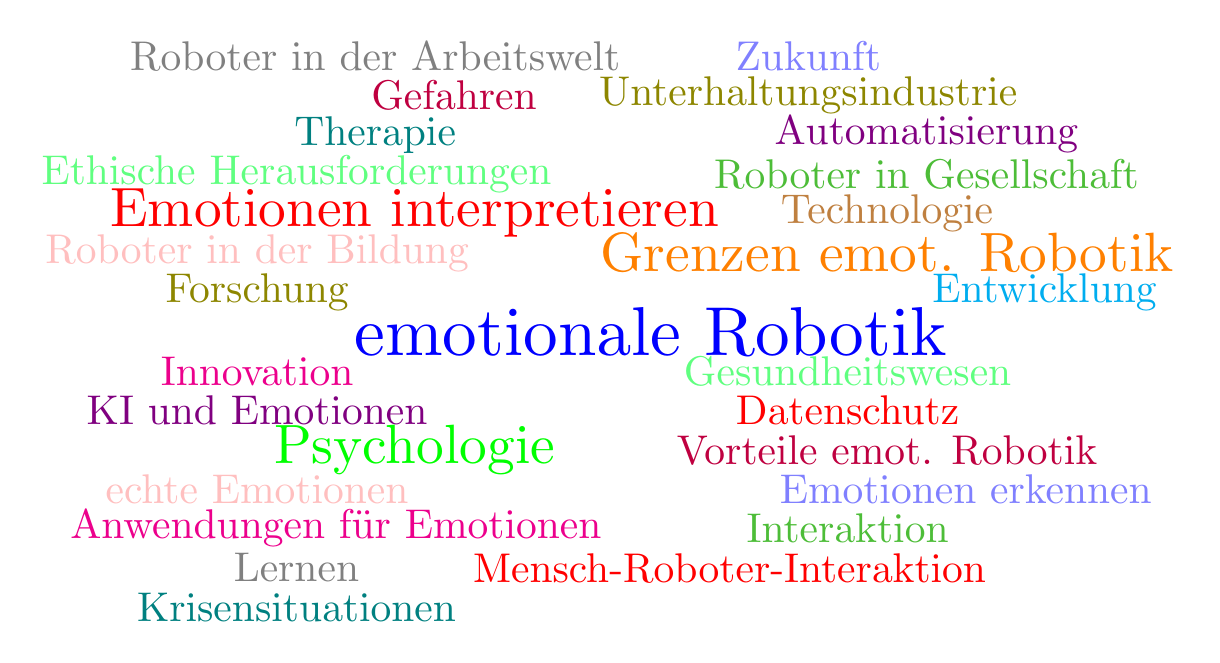
\begin{tikzpicture}[scale=0.5]
      \node at (-7,7) [scale=1.5, color=gray] {Roboter in der Arbeitswelt};
      \node at (4,7) [scale=1.5, color=blue!50!white] {Zukunft};
      \node at (-5,6) [scale=1.5, color=purple] {Gefahren};
      \node at (4,6) [scale=1.5, color=olive] {Unterhaltungsindustrie};
      \node at (-7,5) [scale=1.5, color=teal] {Therapie};
      \node at (7,5) [scale=1.5, color=violet] {Automatisierung};
      \node at (-9,4) [scale=1.5, color=lime!50!cyan] {Ethische Herausforderungen};
      \node at (7,4) [scale=1.5, color=yellow!30!green] {Roboter in Gesellschaft};
      \node at (-6,3) [scale=2, color=red] {Emotionen interpretieren};
      \node at (6,3) [scale=1.5, color=brown] {Technologie};
      \node at (-10,2) [scale=1.5, color=pink] {Roboter in der Bildung};
      \node at (6,2) [scale=2, color=orange] {Grenzen emot. Robotik};
      \node at (-10,1) [scale=1.5, color=olive] {Forschung};
      \node at (10,1) [scale=1.5, color=cyan] {Entwicklung};
      \node at (0,0) [scale=2.5, color=blue] {emotionale Robotik};
      \node at (-10,-1) [scale=1.5, color=magenta] {Innovation};
      \node at (5,-1) [scale=1.5, color=lime!50!cyan] {Gesundheitswesen};
      \node at (-10,-2) [scale=1.5, color=violet] {KI und Emotionen};
      \node at (5,-2) [scale=1.5, color=red] {Datenschutz};
      \node at (-6,-3) [scale=2, color=green] {Psychologie};
      \node at (6,-3) [scale=1.5, color=purple] {Vorteile emot. Robotik};
      \node at (-10,-4) [scale=1.5, color=pink] {echte Emotionen};
      \node at (8,-4) [scale=1.5, color=blue!50!white] {Emotionen erkennen};
      \node at (-8,-5) [scale=1.5, color=magenta] {Anwendungen für Emotionen};
      \node at (5,-5) [scale=1.5, color=yellow!30!green] {Interaktion};
      \node at (2,-6) [scale=1.5, color=red] {Mensch-Roboter-Interaktion};
      \node at (-9,-6) [scale=1.5, color=gray] {Lernen};
      \node at (-9,-7) [scale=1.5, color=teal] {Krisensituationen};
    \end{tikzpicture}
  \end{figure}
\end{frame}

\begin{frame}
  \begin{figure}
    \centering
    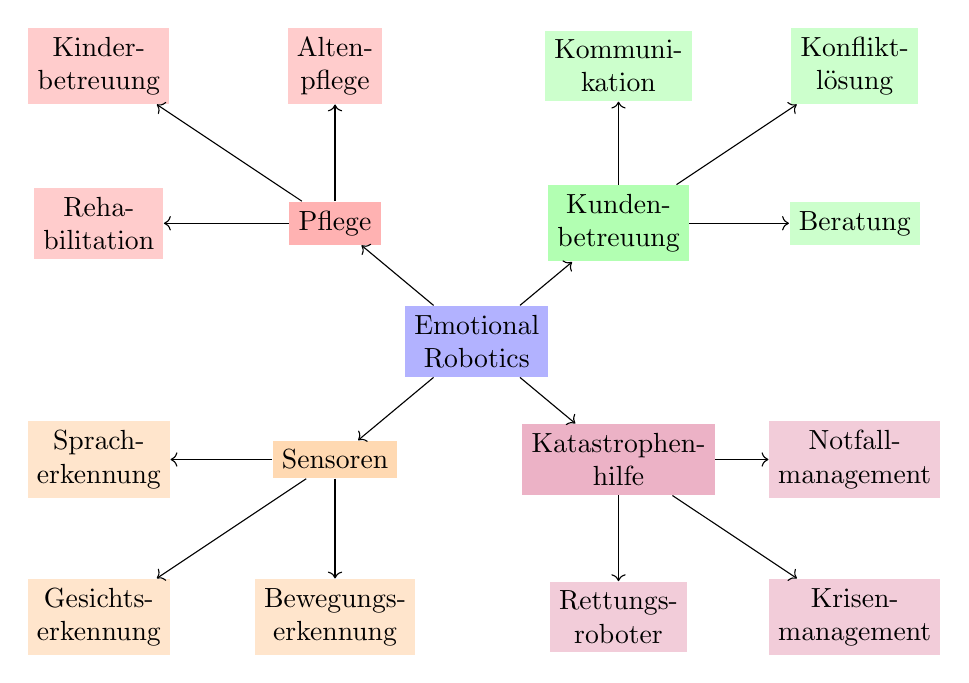
\begin{tikzpicture}[draw, align=center, node distance = 1.5cm and 1.8cm, on grid]
      \begin{scope}[]
        \node (center) [fill=blue!30] {Emotional\\Robotics};
        \node (n1) [above left=of center, fill=red!30]  {Pflege};
        \node (n2) [above right=of center, fill=green!30]  {Kunden-\\betreuung};
        \node (n3) [below left=of center, fill=orange!30]  {Sensoren};
        \node (n4) [below right=of center, fill=purple!30]  {Katastrophen-\\hilfe};

        \node (n11) [left =3cm  of n1, fill=red!20]  {Reha-\\bilitation};
        \node (n12) [above left=2cm  and 3cm  of n1, fill=red!20]  {Kinder-\\betreuung};
        \node (n13) [above =2cm  of n1, fill=red!20]  {Alten-\\pflege};

        \node (n21) [above =2cm of n2, fill=green!20]  {Kommuni-\\kation};
        \node (n22) [above right=2cm  and 3cm  of n2, fill=green!20]  {Konflikt-\\lösung};
        \node (n23) [right =3cm  of  n2, fill=green!20]  {Beratung};

        \node (n31) [below=2cm of n3, fill=orange!20]  {Bewegungs-\\erkennung};
        \node (n32) [below left=2cm  and 3cm  of n3, fill=orange!20]  {Gesichts-\\erkennung};
        \node (n33) [left=3cm  of n3, fill=orange!20]  {Sprach-\\erkennung};

        \node (n41) [below=2cm of n4, fill=purple!20]  {Rettungs-\\roboter};
        \node (n42) [below right=2cm  and 3cm  of n4, fill=purple!20]  {Krisen-\\management};
        \node (n43) [right=3cm  of n4, fill=purple!20]  {Notfall-\\management};

        % Draw arrows from center to next node to outer node
        \draw[->] (center) -- (n1);
        \draw[->] (n1) -- (n11);
        \draw[->] (n1) -- (n12);
        \draw[->] (n1) -- (n13);

        \draw[->] (center) -- (n2);
        \draw[->] (n2) -- (n21);
        \draw[->] (n2) -- (n22);
        \draw[->] (n2) -- (n23);

        \draw[->] (center) -- (n3);
        \draw[->] (n3) -- (n31);
        \draw[->] (n3) -- (n32);
        \draw[->] (n3) -- (n33);

        \draw[->] (center) -- (n4);
        \draw[->] (n4) -- (n41);
        \draw[->] (n4) -- (n42);
        \draw[->] (n4) -- (n43);
      \end{scope}
    \end{tikzpicture}
  \end{figure}
\end{frame}

\begin{frame}[c]{}
  \centering
  \begin{minipage}{\textwidth}
    \usebeamercolor[fg]{normal text}
    \centering
    \Large \atextsl{Alle Folien als CC-BY-SA verfügbar auf}\\
    \href{https://github.com/wieerwill/emotional-robotics}{GitHub.com/WieErWill/emotional-robotics}\\
    \vspace{.4cm}
    \includegraphics[width=.4\linewidth]{images/qrcode-repo.png}
  \end{minipage}
\end{frame}

\begin{frame}[c]{}
  \centering
  \begin{minipage}{\textwidth}
    \usebeamercolor[fg]{normal text}
    \centering
    \Huge Thank You\\
    \Large \atextsl{
      Vielen Dank für eure \\Fragen und Diskussionen
    }
  \end{minipage}
\end{frame}
\end{document}